\let\negthickspace\undefined
\documentclass[journal,12pt,twocolumn]{IEEEtran}
\usepackage{cite}
\usepackage{amsmath,amssymb,amsfonts,amsthm}
\usepackage{algorithmic}
\usepackage{graphicx}
\usepackage{textcomp}
\usepackage{xcolor}
\usepackage{txfonts}
\usepackage{listings}
\usepackage{enumitem}
\usepackage{mathtools}
\usepackage{gensymb}
\usepackage{comment}
\usepackage[breaklinks=true]{hyperref}
\usepackage{tkz-euclide} 
\usepackage{listings}
\usepackage{gvv}                                        
\def\inputGnumericTable{}                                 
\usepackage[latin1]{inputenc}                                
\usepackage{color}                                            
\usepackage{array}                                            
\usepackage{longtable}                                       
\usepackage{calc}                                             
\usepackage{multirow}                                         
\usepackage{hhline}                                           
\usepackage{ifthen}                                           
\usepackage{lscape}
\setlength{\arrayrulewidth}{0.5mm}
\setlength{\tabcolsep}{18pt}
\renewcommand{\arraystretch}{1.5}
\newtheorem{theorem}{Theorem}[section]
\newtheorem{problem}{Problem}
\newtheorem{proposition}{Proposition}[section]
\newtheorem{lemma}{Lemma}[section]
\newtheorem{corollary}[theorem]{Corollary}
\newtheorem{example}{Example}[section]
\newtheorem{definition}[problem]{Definition}
\newcommand{\BEQA}{\begin{eqnarray}}
\newcommand{\EEQA}{\end{eqnarray}}
\newcommand{\define}{\stackrel{\triangle}{=}}
\theoremstyle{remark}
\newtheorem{rem}{Remark}
\begin{document}
\title{Sequence(19) 10.5.3}
\author{EE23BTECH11051-Rajnil Malviya}
\date{January 2024}
\maketitle
\subsection*{\textit{Question :-}}
200 logs are stacked in the following manner: 20 logs in the bottom row, 19 in the next row,
18 in the row next to it and so on . In how many rows are the 200 logs placed
and how many logs are in the top row?

\begin{table}[h!]
   
        \begin{tabular}{ | m{1.0cm} | m{3cm} |m{1cm} |} 
  \hline
 Symbol &Description& Value \\ 
 \hline
$x(0)$&bottom row& 20  \\
\hline
d&common difference & -1  \\
\hline
$S_n$& total number of logs&200 \\
\hline
x(n)&number of logs in n row&  depends on n\\
\hline
\end{tabular}\\
\caption{}
\label{Table:1}
       
    \end{table}
For an Arithmetic Progression :-
\begin{align}x(n)=[x(0)+n d]u(n)\end{align}
\begin{align}x(n)=[20-n]u(n)\end{align}


\begin{align} X(Z)=\frac{20-21z^{-1}}{(1 - z^{-1})^2}  \quad \abs{ z} > 1\end{align}
\begin{align}y(n) = x(n)*u(n)\end{align}
\begin{align}Y(Z) = X(Z)U(Z)\end{align}
\begin{align}Y(Z) = \frac{20-21z^{-1}}{(1 - z^{-1})^3}\end{align}
 Using Contour Integration to find the inverse $Z$-transform,
\begin{align}
    y(n)&=\frac{1}{2\pi j}\oint_{C}Y(z) \;z^{n-1} \;dz  \\
    &=\frac{1}{2\pi j}\oint_{C} \frac{(20-21z^{-1}) z^{n-1}}{(1 - z^{-1})^3} \;dz 
\end{align}
We can observe that the pole is repeated $3$ times and thus $m=3$,
\begin{align}
    R&=\frac{1}{\brak {m-1}!}\lim\limits_{z\to a}\frac{d^{m-1}}{dz^{m-1}}\brak {{(z-a)}^{m}f\brak z}  \\
    &=\frac{1}{\brak {2}!}\lim\limits_{z\to 1}\frac{d^{2}}{dz^{2}}\brak {20 z^{n+2}-21 z^{n+1}}   \\
    &=\frac{1}{2}\lim\limits_{z\to 1}(20(n+2)(n+1)z^{n}-21(n)(n+1)z^{n-1})   \\
    &=\frac{1}{2}[20(n+2)(n+1)-21(n)(n+1)]\end{align}
    \begin{align}
  R=S_n
\end{align}
 \begin{align}
  200=\frac{1}{2}[20(n+2)(n+1)-21(n)(n+1)]
\end{align}
\begin{align}n=15\; ,\;24\end{align}
For Practical reasons \\
x(n) is number of logs in top row
\begin{align}x(n)>0\end{align}
Using equation 2
\begin{align}x(15)=5\end{align}
\begin{align}x(24)=-4 \end{align}
x(24) is rejected because it is negative
\begin{align}x(15)=5\end{align}
Ans. There are 16 rows with 5 logs in top row
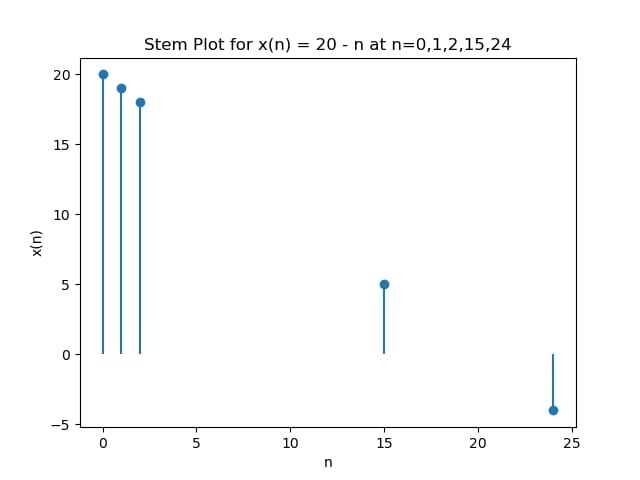
\includegraphics[width=2\linewidth]{figs/f2.png}\\\\

\end{document}
